\documentclass[10pt,aspectratio=169,handout]{beamer}

\usepackage[utf8]{inputenc}
\usepackage[ngerman]{babel}
\usepackage{utopia}
\usetheme{Darmstadt}
\usecolortheme{default}
\usepackage{xcolor}
\usepackage{graphicx}
\usepackage{amsmath}
\usepackage{amsthm}
\usepackage{amssymb}
\usepackage{amsfonts}
\usepackage{mathtools}
\usepackage{dsfont}
\usepackage{hyperref}
\usepackage[most]{tcolorbox}
\usepackage{tikz}
\usepackage{adjustbox}
\usepackage{mathrsfs}
\usepackage{minted}
\usetikzlibrary{cd}
\usetikzlibrary{positioning}
\usetikzlibrary{calc}
\usetikzlibrary{arrows.meta}
\setbeamertemplate{theorems}[numbered]
\setbeamertemplate{navigation symbols}{}
\newtranslation[to=ngerman]{Theorem}{Satz}
\def\C{\mathbb{C}}
\def\R{\mathbb{R}}
\def\Q{\mathbb{Q}}
\def\N{\mathbb{N}}
\def\Z{\mathbb{Z}}
\def\cA{\mathcal{A}}
\definecolor{LightGray}{gray}{0.9}


\begin{document}

\title{Principles of Machine Learning: Exercise 2}
\date{19.11.2023}
\author{Alina Pollehn (3197257), Julian Litz (3362592), Manuel Hinz (3334548)\\
    Felix Göhde (3336445), Felix Lehmann (3177181), Caspar Wiswesser (3221493)\\
    Adrian Köring (3347785), Greta Günther (3326765), Linus Mallwitz (3327653)\\
    Niklas Mueller-Goldingen (3363219), Jennifer Kroppen (2783393)}

\begin{frame}
    \maketitle
\end{frame}

\section{Exercise 2.1}
\begin{frame}
    \frametitle{Task 2.1.1-2}
    Instead of removing the outliers, its easier to keep the inliers:
    \inputminted[bgcolor=LightGray,fontsize=\small]{python}{code/filter-outliers.py}

    Maximum Likelihood Estimation of a Gaussian via empirical mean and covariance:
    \inputminted[bgcolor=LightGray,fontsize=\small]{python}{code/gaussian-mle.py}
\end{frame}

\begin{frame}
    \frametitle{Task 2.1.3}
    Conditional Probability of a Gaussian:
    \inputminted[bgcolor=LightGray,fontsize=\small]{python}{code/predict-gaussian.py}
    
    \begin{columns}
        \begin{column}{0.5\textwidth}
        \begin{center}
            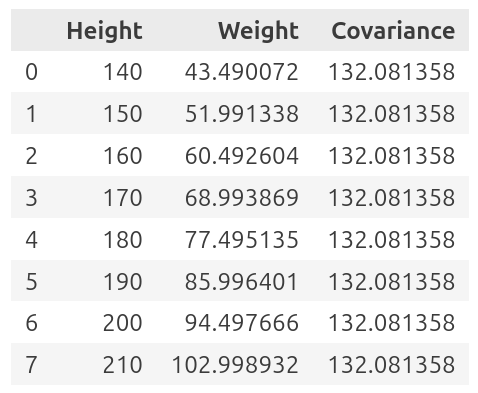
\includegraphics[width=0.7\textwidth]{images/predictions.png}
        \end{center}
        \end{column}
        \begin{column}{0.5\textwidth}  
        \begin{figure}
            \centering
            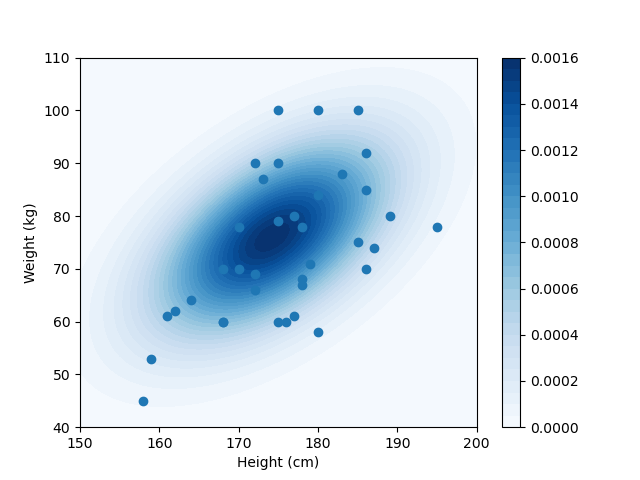
\includegraphics[width=0.7\textwidth]{images/gaussian.png}
            \caption{Estimated PDF and given data}
            \end{figure}
        \end{column}
    \end{columns}
\end{frame}

\begin{frame}
    \frametitle{Task 2.1.3 :: Pondering}

    \begin{itemize}
        \item[+] Results seem plausible -- mostly so around the mean
        \item[-] Fixed variance doesnt match expectations (taller people $\rightarrow$ more variance)
        \item[-] Cube-Square-Law suggests a non-linear relationship?
        \item    Plausibility? Test-Set!
    \end{itemize}
\end{frame}

\section{2.2}
\begin{frame}
    \frametitle{Task 2.2.1}
    % Conditional Probability of a Gaussian:
    % \inputminted[bgcolor=LightGray,fontsize=\small]{python}{code/predict-gaussian.py}
    
    % \begin{columns}
    %     \begin{column}{0.5\textwidth}
    %     \begin{center}
    %         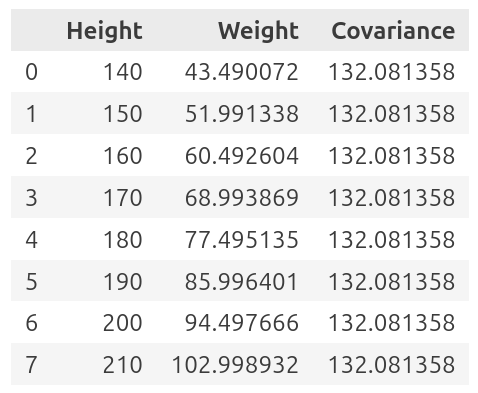
\includegraphics[width=0.7\textwidth]{images/predictions.png}
    %     \end{center}
    %     \end{column}
    %     \begin{column}{0.5\textwidth}  
    %     \begin{figure}
    %         \centering
    %         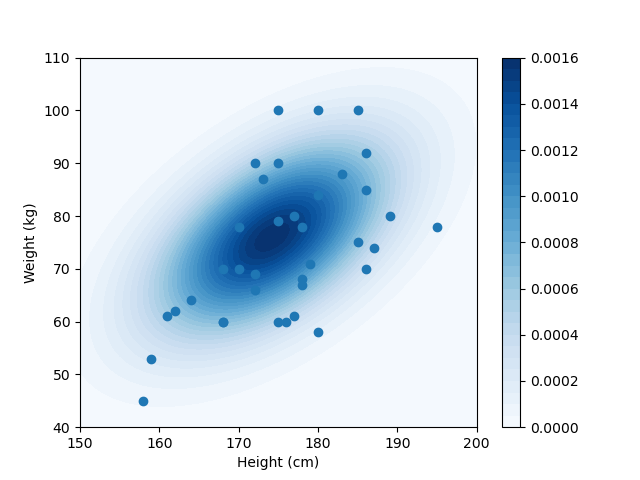
\includegraphics[width=0.7\textwidth]{images/gaussian.png}
    %         \caption{Estimated PDF and given data}
    %         \end{figure}
    %     \end{column}
    % \end{columns}
\end{frame}

\section{2.3}
\begin{frame}
    \frametitle{Task 2.3}
\end{frame}

\section{2.4}
\begin{frame}
    \frametitle{Task 2.4}
\end{frame}

\section{2.5}
\begin{frame}
    \frametitle{Task 2.5}
\end{frame}

\end{document}
